\documentclass{article}
\usepackage[utf8]{inputenc}
\usepackage{tikz}
\usetikzlibrary{shapes, arrows.meta, positioning}

\title{Taller de Bases de Datos}
\author{Carlos Padilla}
\date{\today}

\begin{document}

\maketitle

\section{Mapa Conceptual de Gestores de Bases de Datos}

\begin{center}
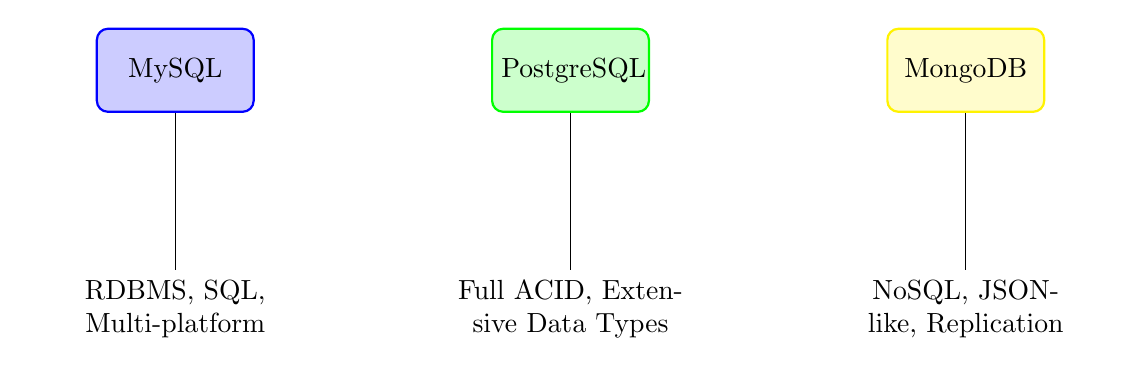
\begin{tikzpicture}[node distance=2cm and 3cm, auto]
  \node (mysql) [rectangle, draw=blue, thick, fill=blue!20, text width=5em, text centered, rounded corners, minimum height=3em] {MySQL};
  \node (postgres) [rectangle, draw=green, thick, fill=green!20, right=of mysql, text width=5em, text centered, rounded corners, minimum height=3em] {PostgreSQL};
  \node (mongodb) [rectangle, draw=yellow, thick, fill=yellow!20, right=of postgres, text width=5em, text centered, rounded corners, minimum height=3em] {MongoDB};

  \node (rdbms) [below= of mysql, text width=10em, text centered] {RDBMS, SQL, Multi-platform};
  \node (acid) [below= of postgres, text width=10em, text centered] {Full ACID, Extensive Data Types};
  \node (nosql) [below= of mongodb, text width=10em, text centered] {NoSQL, JSON-like, Replication};

  \path[-] (mysql) edge (rdbms);
  \path[-] (postgres) edge (acid);
  \path[-] (mongodb) edge (nosql);
\end{tikzpicture}
\end{center}

\end{document}

